\documentclass[10pt]{article}

\usepackage[margin=0.75in]{geometry}
\usepackage{amsmath, amssymb}
\usepackage{graphicx}
\usepackage[T1]{fontenc}
\usepackage{inconsolata}
\usepackage{titlesec}
\usepackage{fancyhdr}
\usepackage{microtype}
\usepackage{tikz}
\usetikzlibrary{arrows.meta}

\graphicspath{{../}}

\setlength{\parindent}{0pt}
\setlength{\parskip}{4pt}
\renewcommand{\baselinestretch}{1.05}

\titleformat{\section}{\ttfamily\normalsize\bfseries\MakeUppercase}{\thesection}{0.6em}{}
\titlespacing*{\section}{0pt}{8pt}{2pt}
\titleformat{\subsection}{\ttfamily\small\MakeUppercase}{\thesubsection}{0.6em}{}
\titlespacing*{\subsection}{0pt}{6pt}{2pt}

\pagestyle{fancy}
\fancyhf{}
\renewcommand{\headrulewidth}{0pt}
\renewcommand{\footrulewidth}{0.5pt}
\fancyfoot[L]{\ttfamily\footnotesize PLATE-SLAB-METHODOLOGY}
\fancyfoot[C]{\ttfamily\footnotesize REV \today}
\fancyfoot[R]{\ttfamily\footnotesize \thepage}

\begin{document}

\noindent
\includegraphics[height=0.7cm]{logo}\hfill
{\ttfamily\normalsize\bfseries\MakeUppercase{SET Plate-Slab Methodology}}\quad
{\ttfamily\footnotesize\today}
\vspace{4pt}\hrule\vspace{6pt}

\section{Design Baseline}

\medskip{\ttfamily\footnotesize\bfseries SLAB SELECTION MATRIX}

{\ttfamily\footnotesize
\renewcommand{\arraystretch}{1.2}
\begin{tabular}{@{}p{0.55in}p{1.15in}p{1.15in}p{0.95in}p{0.95in}p{0.95in}@{}}
Slab & Top bars (X+Y) & Bottom bars (X+Y) & Ext. span & Int. span & Shear studs? \\
\hline
8 in & \#5 @ 12 in O.C. & \#4 @ 12 in O.C. & 20'-0" & 22'-0" & @ roof / rare \\
9 in & \#5 @ 12 in O.C.* & \#5 @ 12 in O.C. & 22'-6" & 24'-9" & yes \\
10 in & \#5 @ 12 in O.C.* & \#5 @ 12 in O.C. & 25'-0" & 27'-6" & yes \\
11 in & \#5 @ 12 in O.C.* & \#5 @ 12 in O.C. & 27'-6" & 30'-3" & yes \\
12 in & \#5 @ 12 in O.C.* & \#6 @ 12 in O.C. & 30'-0" & 33'-0" & yes \\
\end{tabular}
}

\vspace{1pt}{\ttfamily\tiny * BASE MAT; ADD COLUMN-STRIP TOP STEEL PER DESIGN.}

\vspace{1pt}{\ttfamily\tiny COLUMNS: 12 x 24 in DEFAULT; 10 in DIAMETER OR 10 x 30 in PROJECT-SPECIFIC.}

\medskip{\ttfamily\footnotesize\bfseries LOAD BASIS}

\begin{equation}
\begin{aligned}
w_{\mathrm{sw},8} &= 100\ \text{psf},
& w_{\mathrm{SDL}} &= 35\ \text{psf},
& D_8 &= w_{\mathrm{sw},8}+w_{\mathrm{SDL}}=135\ \text{psf} \\
L &= 40\ \text{psf},
& w_{u,8} &= 1.2D_8 + 1.6L = 226\ \text{psf}
\end{aligned}
\end{equation}

{\ttfamily\footnotesize
\begin{tabular}{@{}ll@{}}
$w_{\mathrm{sw},8}$ & 8 in slab self-weight, 100 psf \\
$w_{\mathrm{SDL}}$ & superimposed dead load, 35 psf \\
$D_8$ & total unfactored dead load for the 8 in slab, 135 psf \\
$w_{u,8}$ & factored typical-floor area load for the 8 in slab \\
$L$ & unfactored live area load, 40 psf \\
\end{tabular}
}

\medskip{\ttfamily\footnotesize\bfseries TYPICAL 3 BY 3 BAY LAYOUT}

\begin{center}
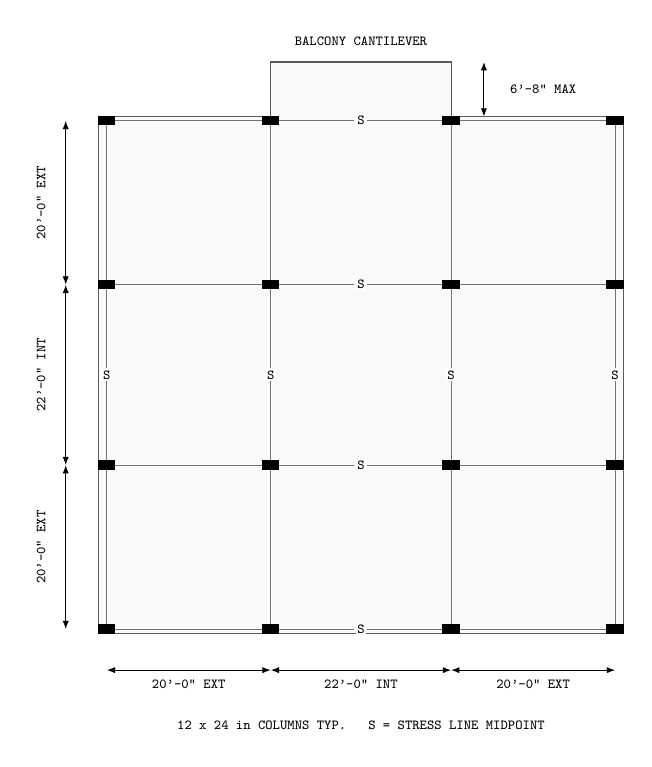
\begin{tikzpicture}[
  x=0.041in,
  y=0.041in,
  slab/.style={fill=black!2,draw=black!65,line width=0.45pt},
  stress/.style={draw=black!55,line width=0.35pt},
  column/.style={fill=black,draw=black},
  dim/.style={{Latex[length=3pt]}-{Latex[length=3pt]},thin},
  lab/.style={font=\ttfamily\tiny},
  smark/.style={font=\ttfamily\tiny\bfseries,fill=white,inner sep=0.6pt}
]
\path[slab]
  (-1,-0.5) -- (63,-0.5) -- (63,62.5) --
  (42,62.5) -- (42,69.167) -- (20,69.167) --
  (20,62.5) -- (-1,62.5) -- cycle;
\foreach \y in {0,20,42,62} {
  \draw[stress] (0,\y) -- (30.2,\y);
  \draw[stress] (31.8,\y) -- (62,\y);
  \node[smark] at (31,\y) {S};
}
\foreach \x in {0,20,42,62} {
  \draw[stress] (\x,0) -- (\x,30.2);
  \draw[stress] (\x,31.8) -- (\x,62);
  \node[smark] at (\x,31) {S};
}
\foreach \x in {0,20,42,62} {
  \foreach \y in {0,20,42,62} {
    \path[column] (\x-1,\y-0.5) rectangle (\x+1,\y+0.5);
  }
}

\draw[dim] (0,-5) -- (20,-5) node[midway,below,lab]{20'-0" EXT};
\draw[dim] (20,-5) -- (42,-5) node[midway,below,lab]{22'-0" INT};
\draw[dim] (42,-5) -- (62,-5) node[midway,below,lab]{20'-0" EXT};

\draw[dim] (-5,0) -- (-5,20);
\draw[dim] (-5,20) -- (-5,42);
\draw[dim] (-5,42) -- (-5,62);
\node[lab,rotate=90] at (-8,10) {20'-0" EXT};
\node[lab,rotate=90] at (-8,31) {22'-0" INT};
\node[lab,rotate=90] at (-8,52) {20'-0" EXT};

\draw[dim] (46,62.5) -- (46,69.167);
\node[lab,anchor=west] at (48,65.8335) {6'-8" MAX};
\node[lab,above] at (31,70) {BALCONY CANTILEVER};
\node[lab,below] at (31,-10) {12 x 24 in COLUMNS TYP. \quad S = STRESS LINE MIDPOINT};
\end{tikzpicture}
\end{center}

\begin{equation}
h \ge \frac{L_b}{10}
\qquad \Rightarrow \qquad
L_b \le 10h = 80\ \text{in} = \text{6'-8"}
\end{equation}

{\ttfamily\footnotesize
\begin{tabular}{@{}ll@{}}
$h$ & slab thickness, 8 in \\
$L_b$ & balcony cantilever length \\
\end{tabular}
}

\medskip{\ttfamily\footnotesize\bfseries CONTROLLING BALCONY LIMIT: 6'-8" MAX}

\clearpage
\section{Proof for Gabe (Temporary)}

\medskip{\ttfamily\footnotesize\bfseries GOAL}

Determine workable exterior and interior spans for 9, 10, 11, and 12 in
conventionally reinforced plate slabs under confirmed SET criteria.

\medskip{\ttfamily\footnotesize\bfseries ACI 318-19 SPAN CONTROL}

\begin{equation}
\ell_{n,e}\leq30h,
\qquad
\ell_{n,i}\leq33h,
\qquad
L_b\leq10h
\end{equation}

{\ttfamily\footnotesize
\begin{tabular}{@{}ll@{}}
$\ell_{n,e}$ & clear exterior span without an edge beam [in] \\
$\ell_{n,i}$ & clear interior span [in] \\
$h$ & slab thickness [in] \\
$L_b$ & balcony cantilever length [in] \\
\end{tabular}
}

\medskip{\ttfamily\footnotesize\bfseries LIMIT BASIS}

{\ttfamily\footnotesize
\begin{tabular}{@{}p{1.65in}p{5.05in}@{}}
Reference & ACI 318-19 Table 8.3.1.1; Grade 60; no drop panels \\
Exterior & no edge beam; $h\geq\ell_{n,e}/30$ \\
Interior & $h\geq\ell_{n,i}/33$ \\
Grid convention & listed grid span $\geq$ actual clear span; conservative \\
\end{tabular}
}

\medskip{\ttfamily\footnotesize\bfseries WORKABLE SPAN SCREEN}

{\ttfamily\footnotesize
\renewcommand{\arraystretch}{1.2}
\begin{tabular}{@{}l@{\hspace{0.50in}}l@{\hspace{0.65in}}l@{\hspace{0.65in}}l@{\hspace{0.60in}}l@{}}
Slab & Exterior & Interior & Balcony & Status \\
\hline
8 in  & 20'-0" & 22'-0" & 6'-8"  & accepted baseline \\
9 in  & 22'-6" & 24'-9" & 7'-6"  & workable + studs \\
10 in & 25'-0" & 27'-6" & 8'-4"  & workable + studs \\
11 in & 27'-6" & 30'-3" & 9'-2"  & workable + studs \\
12 in & 30'-0" & 33'-0" & 10'-0" & workable + studs \\
\end{tabular}
}

\medskip{\ttfamily\footnotesize\bfseries DEEPER-SLAB LOAD DEPENDENCY}

\begin{equation}
w_{\mathrm{sw},h}=\gamma_c
\left(\frac{h}{12\ \text{in/ft}}\right),
\qquad
D_h=w_{\mathrm{sw},h}+w_{\mathrm{SDL}},
\qquad
w_{u,h}=1.2D_h+1.6L
\end{equation}

{\ttfamily\footnotesize
\begin{tabular}{@{}ll@{}}
$w_{\mathrm{sw},h}$ & slab self-weight for trial slab thickness $h$ [psf] \\
$D_h$ & unfactored dead area load for trial slab thickness $h$ \\
$w_{\mathrm{SDL}}$ & superimposed dead load, 35 psf \\
$\gamma_c$ & concrete unit weight, 150 pcf \\
$w_{u,h}$ & factored area load for trial slab thickness $h$ [psf] \\
\end{tabular}
}

\medskip{\ttfamily\footnotesize\bfseries FACTORED LOADS}

{\ttfamily\footnotesize
\renewcommand{\arraystretch}{1.15}
\begin{tabular}{@{}p{0.70in}p{1.10in}p{0.95in}p{1.10in}p{1.10in}@{}}
Slab & $w_{\mathrm{sw},h}$ & $w_{\mathrm{SDL}}$ & $D_h$ & $w_{u,h}$ \\
\hline
8 in  & 100.0 psf & 35 psf & 135.0 psf & 226 psf \\
9 in  & 112.5 psf & 35 psf & 147.5 psf & 241 psf \\
10 in & 125.0 psf & 35 psf & 160.0 psf & 256 psf \\
11 in & 137.5 psf & 35 psf & 172.5 psf & 271 psf \\
12 in & 150.0 psf & 35 psf & 185.0 psf & 286 psf \\
\end{tabular}
}

\medskip{\ttfamily\footnotesize\bfseries CONFIRMED BASIS}

{\ttfamily\footnotesize
\begin{tabular}{@{}p{1.65in}p{5.05in}@{}}
Code & ACI 318-19 \\
Concrete strength & $f'_c=5$ ksi \\
Steel strength & $f_y=60$ ksi \\
Concrete unit weight & $\gamma_c=150$ pcf; normalweight \\
Superimposed dead load & $w_{\mathrm{SDL}}=35$ psf \\
Clear cover & $c_{\text{clr}}=0.75$ in \\
\end{tabular}
}

\medskip{\ttfamily\footnotesize\bfseries SHORING}

{\ttfamily\footnotesize
\begin{tabular}{@{}p{1.45in}@{\hspace{0.18in}}p{5.05in}@{}}
Thickness trigger & none; slab thickness alone does not determine reshoring \\
12 in shoring case & 150 psf fresh-concrete slab self-weight; add formwork and construction live loads \\
8 to 12 in slabs & shore during placement; reshore per engineered construction plan \\
Release criterion & verified in-place strength + construction-load capacity; not age alone \\
Required inputs & pour cycle; supported levels; slab age and strength; fresh concrete, formwork, worker, and equipment loads; shore spacing and stiffness \\
Reference & ACI PRC-347.2-17(25) \\
\end{tabular}
}

\clearpage
\medskip{\ttfamily\footnotesize\bfseries ACI DIRECT-DESIGN APPLICABILITY}

{\ttfamily\footnotesize
\begin{tabular}{@{}p{2.15in}p{4.55in}@{}}
Continuous spans & three in each direction; pass \\
Adjacent-span ratio & $L_i/L_e=1.10\leq1.20$; pass \\
Panel aspect ratio & 1.00 $\leq$ 2.00; pass \\
Column offset & zero; pass \\
Live-to-dead ratio & $L/D_8=0.30\leq2.00$; pass \\
\end{tabular}
}

\medskip{\ttfamily\footnotesize\bfseries INTERIOR-PANEL MOMENT SCREEN}

\begin{equation}
\ell_n=L_i-12\ \text{in},
\qquad
\ell_2=L_i,
\qquad
M_o=\frac{w_{u,h}\ell_2\ell_n^2}{8}
\end{equation}

\begin{equation}
m_u^+=\frac{2(0.60)(0.35)M_o}{\ell_2}
=\frac{0.42M_o}{\ell_2},
\qquad
m_u^-=\frac{2(0.75)(0.65)M_o}{\ell_2}
=\frac{0.975M_o}{\ell_2}
\end{equation}

{\ttfamily\footnotesize
\begin{tabular}{@{}ll@{}}
$L_e$ & listed exterior grid span [ft] \\
$L_i$ & listed interior grid span [ft] \\
$\ell_n$ & governing interior clear span using the 12 in column side [ft] \\
$\ell_2$ & transverse panel width [ft] \\
$M_o$ & total static factored moment [kip-ft] \\
$m_u^+$ & positive column-strip factored moment per foot [kip-ft/ft] \\
$m_u^-$ & negative column-strip factored moment per foot [kip-ft/ft] \\
\end{tabular}
}

\medskip{\ttfamily\footnotesize\bfseries FLEXURAL STRENGTH}

\begin{equation}
a=\frac{A_s f_y}{0.85f'_c b},
\qquad
\phi_f m_n=\frac{\phi_f A_s f_y}{12}
\left(d_f-\frac{a}{2}\right),
\qquad
\phi_f=0.90
\end{equation}

{\ttfamily\footnotesize
\begin{tabular}{@{}ll@{}}
$a$ & equivalent compression-block depth [in] \\
$A_s$ & flexural reinforcement per foot [in$^2$/ft] \\
$f_y$ & reinforcement yield strength, 60 ksi \\
$b$ & design-strip width, 12 in \\
$m_n$ & nominal flexural strength per foot [kip-ft/ft] \\
$d_f$ & effective flexural depth to governing inner bar layer [in] \\
$\phi_f$ & flexural strength-reduction factor, 0.90 \\
\end{tabular}
}

\medskip{\ttfamily\footnotesize\bfseries POSITIVE-MOMENT BOTTOM MAT}

{\ttfamily\footnotesize
\renewcommand{\arraystretch}{1.15}
\begin{tabular}{@{}p{0.55in}p{0.85in}p{1.20in}p{0.95in}p{0.70in}p{1.00in}@{}}
Slab & $m_u^+$ & Bottom mat & $\phi_fm_n$ & DCR & $A_{s,\min}$ \\
\hline
9 in  & 7.14 & \#5 @ 12 in O.C. & 9.95 & 0.72 & pass \\
10 in & 9.44 & \#5 @ 12 in O.C. & 11.34 & 0.83 & pass \\
11 in & 12.17 & \#5 @ 12 in O.C. & 12.74 & 0.96 & pass \\
12 in & 15.38 & \#6 @ 12 in O.C. & 19.54 & 0.79 & pass \\
\end{tabular}
}

\vspace{2pt}{\ttfamily\tiny DCR $=m_u^+/(\phi_fm_n)$; $A_{s,\min}=0.0018bh$;
$A_{s,\min}$ = MINIMUM SLAB REINFORCEMENT PER FOOT.}

\medskip{\ttfamily\footnotesize\bfseries NEGATIVE-MOMENT COLUMN STRIP}

{\ttfamily\footnotesize
\renewcommand{\arraystretch}{1.15}
\begin{tabular}{@{}p{0.55in}p{0.85in}p{2.25in}p{0.75in}p{0.95in}p{0.70in}@{}}
Slab & $m_u^-$ & Trial top steel & $A_s$ & $\phi_fm_n$ & DCR \\
\hline
9 in  & 16.57 & \#5 @ 12 in O.C. + \#4 @ 10 in O.C. & 0.550 & 17.30 & 0.96 \\
10 in & 21.91 & \#5 @ 12 in O.C. + \#5 @ 12 in O.C. & 0.620 & 22.17 & 0.99 \\
11 in & 28.26 & \#5 @ 12 in O.C. + \#6 @ 12 in O.C. & 0.750 & 29.31 & 0.96 \\
12 in & 35.69 & \#5 @ 12 in O.C. + \#7 @ 12 in O.C. & 0.910 & 38.50 & 0.93 \\
\end{tabular}
}

\medskip{\ttfamily\footnotesize\bfseries FLEXURE RESULT: PASS WITH LISTED MATS + TRIAL COLUMN-STRIP TOP STEEL}

\clearpage
\medskip{\ttfamily\footnotesize\bfseries INTERIOR-COLUMN PUNCHING GEOMETRY}

\begin{equation}
d_v=h-c_{\text{clr}}-d_b,
\qquad
A_t=\left(\frac{L_e+L_i}{2}\right)^2,
\qquad
A_o=\frac{(C_x+d_v)(C_y+d_v)}{144}
\end{equation}

\begin{equation}
V_u=w_{u,h}(A_t-A_o),
\qquad
b_o=2(C_x+C_y+2d_v),
\qquad
v_{u,0}=\frac{V_u}{b_od_v}
\end{equation}

{\ttfamily\footnotesize
\begin{tabular}{@{}ll@{}}
$d_v$ & average effective depth for punching [in] \\
$c_{\text{clr}}$ & clear cover, 0.75 in \\
$d_b$ & governing top support-bar diameter [in] \\
$A_t$ & interior-column tributary area [ft$^2$] \\
$A_o$ & area inside the critical perimeter [ft$^2$] \\
$C_x,C_y$ & column dimensions, 12 and 24 in \\
$V_u$ & direct factored shear across the critical perimeter [lb] \\
$b_o$ & critical perimeter at $d_v/2$ from column faces [in] \\
$v_{u,0}$ & direct factored punching stress [psi] \\
\end{tabular}
}

\medskip{\ttfamily\footnotesize\bfseries GRAVITY MOMENT TRANSFER}

\begin{equation}
v_{u,\max}=v_{u,0}
+\frac{\gamma_{vx}M_{ux}y_c}{J_{cx}}
+\frac{\gamma_{vy}M_{uy}x_c}{J_{cy}}
\end{equation}

{\ttfamily\footnotesize
\begin{tabular}{@{}ll@{}}
$v_{u,\max}$ & maximum factored punching stress [psi] \\
$M_{ux},M_{uy}$ & DDM gravity span-imbalance moments [lb-in] \\
$\gamma_{vx},\gamma_{vy}$ & fractions transferred by eccentricity of shear \\
$x_c,y_c$ & critical-section centroid-to-perimeter distances [in] \\
$J_{cx},J_{cy}$ & critical-section properties for moment transfer [in$^4$] \\
\end{tabular}
}

\medskip{\ttfamily\footnotesize\bfseries CONCRETE PUNCHING STRENGTH}

\begin{equation}
\lambda_s=\min\left(1,\sqrt{\frac{2}{1+d_v/(10\ \text{in})}}\right),
\qquad
\phi_vv_c=\phi_v\,4\lambda_s\sqrt{f'_c},
\qquad
\phi_v=0.75
\end{equation}

{\ttfamily\footnotesize
\begin{tabular}{@{}ll@{}}
$\lambda_s$ & ACI size-effect factor, $d_v$ in inches \\
$v_c$ & nominal concrete punching strength [psi] \\
$f'_c$ & specified concrete strength, 5000 psi \\
$\phi_v$ & shear strength-reduction factor, 0.75 \\
\end{tabular}
}

\medskip{\ttfamily\footnotesize\bfseries PUNCHING SCREEN}

{\ttfamily\footnotesize
\renewcommand{\arraystretch}{1.15}
\begin{tabular}{@{}l@{\hspace{0.30in}}r@{\hspace{0.42in}}r@{\hspace{0.42in}}r@{\hspace{0.42in}}r@{\hspace{0.42in}}r@{\hspace{0.42in}}l@{}}
Slab & $d_v$ & $v_{u,0}$ & $v_{u,\max}$ & $\phi_vv_c$ & DCR & Studs \\
\hline
8 in  & 6.625 & 151 psi & 193 psi & 212 psi & 0.91 & @ roof / rare \\
9 in  & 7.625 & 171 psi & 222 psi & 212 psi & 1.05 & yes \\
10 in & 8.625 & 191 psi & 252 psi & 212 psi & 1.19 & yes \\
11 in & 9.500 & 215 psi & 288 psi & 212 psi & 1.36 & yes \\
12 in & 10.375 & 240 psi & 327 psi & 210 psi & 1.56 & yes \\
\end{tabular}
}

\vspace{2pt}{\ttfamily\tiny DCR $=v_{u,\max}/(\phi_vv_c)$; DEMAND/CAPACITY RATIO.}

\begin{equation}
v_{u,\max}\leq8\phi_v\sqrt{f'_c}=424\ \text{psi}
\end{equation}

\medskip{\ttfamily\footnotesize\bfseries STUD FEASIBILITY: PASS; MAXIMUM SCREENED DEMAND = 327 PSI}

\medskip{\ttfamily\footnotesize\bfseries PROOF RESULT}\par

{\ttfamily\footnotesize
\begin{tabular}{@{}p{1.30in}p{5.40in}@{}}
Span/depth & pass per ACI 318-19 Table 8.3.1.1 \\
Deflection & prescriptive thickness control used; calculation not required \\
Flexure & pass with listed bottom mats and trial top column-strip steel \\
Punching & 9--12 in options require studs; inner compression cap passes \\
Result & listed 9--12 in exterior and interior spans are workable \\
Final design & size stud rails; check outer, edge, and corner critical sections \\
\end{tabular}
}

\medskip{\ttfamily\footnotesize\bfseries TEMPORARY PROOF --- REMOVE AFTER GABE REVIEW}

\end{document}
